% ---------------------------------------------------------------------------
% DRAFT. The dam-break matrix and the w_U sweep are complete; Phases 2 and 3
% of the project (the pointwise condition-number diagnostic and the
% Navier-Stokes cases) are not started, so contributions C4 and C5 of the
% proposal have no section here yet. Every citation in references.bib still
% needs verifying by hand. Build with: tectonic -X compile main.tex
% ---------------------------------------------------------------------------
\documentclass[11pt]{article}

\usepackage[english]{babel}
\usepackage{amsmath, amssymb}
\usepackage{booktabs}
\usepackage{graphicx}
\graphicspath{{figures/}}
\usepackage[colorlinks=true, allcolors=blue]{hyperref}
\usepackage[margin=2.5cm]{geometry}
\usepackage{authblk}

\newcommand{\DU}{D}
\newcommand{\wU}{w_U}

\title{\textbf{Spectral weight control in physics-informed neural networks:
what the orthogonality penalty does, and how it transfers to shock-dominated
shallow-water flow}}

\author[1]{Michael Ajao-Olarinoye}
\author[2]{M. Asif Farooq}
\affil[1]{Coventry University, UK}
\affil[2]{National University of Sciences and Technology, Islamabad, Pakistan}

\date{Draft --- \today}

\begin{document}
\maketitle

\begin{abstract}
Wang et al.~\cite{wang2026cnpinn} improve physics-informed neural network
accuracy by factorising each hidden weight at initialisation, training the
left factor and the singular values in place of the weight, and penalising
departures of the left factor from orthogonality with a hand-tuned weight
$\wU$. Their account assigns the gain to control over the weight spectrum. We
reproduce their advection case over 20 seeds and then measure the trained
factors, which their paper does not report. At the published
$\wU = 1/35000$ the trained left factor is not close to orthogonal ---
$\|U^\top U - I\|_2$ has median $0.98$, indicating a collapsed
eigendirection --- and the trained singular values differ from the effective
weight's actual singular values by up to a factor of 13. Constraining the
factor to be exactly orthogonal, which removes $\wU$ entirely, reaches only
$1.7\times10^{-2}$ median relative error against the penalty's
$8.4\times10^{-3}$; removing the penalty from the same parameterisation
returns the error to $2.1\times10^{-1}$, worse than an unconstrained
network's $8.4\times10^{-2}$. Reading the term as a bound on the factor's
scale predicts that a weaker bound should also work; we test that by pinning
only $\sigma_{\max}(U)$, and it is the worst regime of the six at
$3.7\times10^{-1}$ median, so what the penalty supplies is a pull of the whole
spectrum toward 1 rather than a bound on scale. Transferring the comparison to
two-dimensional shallow-water dam breaks, where the solution carries a shock
and the bounded-gradient hypothesis of the source paper's Theorem 2.1 fails,
no spectral regime separates from an unmodified network by more than about
10\% in $L^1$ depth error on the three shock cases, and $\wU$ can be moved
three decades without measurable effect. On the one smooth initial condition
in the set, exact orthogonality and spectrum-only training are a factor of
$2.5$ worse than an unmodified network. Establishing this required checking
our finite-volume reference against an independently implemented solver
family, which disagrees with it by more than the differences under test on
two of three benchmarks --- a floor that comparisons of this kind do not
usually report.
\end{abstract}

\section{Introduction}

Physics-informed neural networks solve a PDE by minimising its residual at
collocation points~\cite{raissi2019pinn}. They fail on targets with steep or
high-frequency structure, and a line of work attributes the failure to
properties of the network's Jacobian. Wang et al.~\cite{wang2026cnpinn}
formalise this through a quantity they call the condition number,
$\kappa(f) = \|J(f)\|_F$, and propose a remedy: decompose each hidden weight
$W_j = U_j S_j V_j^\top$ once at initialisation, freeze $V_j$, train $U_j$ and
$\mathrm{diag}(S_j)$ in place of $W_j$, and add
\begin{equation}
  \wU \sum_j \DU_j^2, \qquad \DU_j = \|U_j^\top U_j - I\|_2
  \label{eq:penalty}
\end{equation}
to the loss so that $U_j$ stays orthogonal and $\mathrm{diag}(S_j)$ therefore
carries the weight's spectrum.

Their conclusion lists three open problems. The penalty weight $\wU$ is tuned
per equation across two and a half decades, from $1/600$ to $1/200000$ over
five PDEs, and their Section 4.6.3 reports that NTK- and DB-PINN-style
adaptive weighting diverges on this term because the penalty starts at exactly
zero. The penalty costs 1.28 to 1.83 times vanilla training time across their
width and collocation sweeps. All five validation problems are, in their own
description, controlled synthetic examples, and all five are smooth.

That last point has a specific consequence. Every hypothesis of their Theorem
2.1 requires $u \in H^1$ with $\|J(u)\|_F$ bounded. A dam-break solution
carries a shock, so $\|J(u)\|_F$ is unbounded and $u \notin H^1$: the theorem
is formally inapplicable to the entire problem class. The authors say as much
in a different context, noting that the condition is violated once training
collapses.

We take the three limitations in order and add the excluded regime.
Section~\ref{sec:mechanism} reproduces the advection case and then measures
what the penalty does to the trained factors, which decides what kind of
constraint the term is. Section~\ref{sec:swe} moves the same weight regimes
to two-dimensional shallow-water dam breaks.
Section~\ref{sec:refcheck} reports a result we did not set out to find: on two of three benchmarks the reference against which all of this is
measured is less certain than the differences being measured.

\section{The parameterisation and the regimes compared}

Write a hidden layer's weight as $W \in \mathbb{R}^{m\times n}$ and its
initial factorisation as $W_0 = U_0 S_0 V_0^\top$. All regimes below keep
$V = V_0$ frozen and differ in how $U$ and the spectrum are treated. A fifth,
introduced in Section~\ref{sec:bounded} once the measurements motivate it,
bounds $U$'s largest singular value.

\begin{description}
  \item[Unconstrained.] $W$ trained directly. The baseline.
  \item[Penalised spectral.] $U$ and $s = \mathrm{diag}(S)$ trained, with
    Eq.~\eqref{eq:penalty} added to the loss. This is the published method.
  \item[Exactly orthogonal.] $U$ constrained to the Stiefel manifold by the
    matrix-exponential parameterisation of Lezcano-Casado and
    Mart\'inez-Rubio~\cite{lezcano2019orthogonal}, and $s$ trained. The
    penalty and $\wU$ do not exist in this regime, which is what makes it the
    direct test of the first stated limitation.
  \item[Spectrum only.] $U$ and $V$ both frozen at their orthogonal initial
    values, $s$ alone trained. Structurally this layer is the one used by
    SVD-PINNs~\cite{gao2022svdpinn}; there it transfers a trained network to a
    new equation, whereas here it is trained from scratch. The construction is
    not ours and is not presented as new.
\end{description}

The distinction between the second and third regimes is the paper's pivot. If
the penalty is an approximation to orthogonality, then enforcing orthogonality
exactly should do at least as well and costs no tuned weight. If it is
something else, the two will separate.


\section{Related work}
\label{sec:related}

\paragraph{Spectral structure in network weights.}
Spectral normalisation~\cite{miyato2018spectral} divides a weight by its
largest singular value to force a 1-Lipschitz map. It acts on the same object
as the method studied here and with the opposite intent: it caps the gradient
magnitude a network can express, whereas the diagnostic
motivating~\cite{wang2026cnpinn} holds that networks fail on steep targets by
expressing too little of it. The exactly-orthogonal regime we test uses the
matrix-exponential parametrisation of Lezcano-Casado and
Mart\'inez-Rubio~\cite{lezcano2019orthogonal}, introduced for recurrent
networks; we are not aware of a prior application to PINN training, and the
result in Section~\ref{sec:mechanism} suggests why one might not have been
reported. SVD-PINNs~\cite{gao2022svdpinn} freeze both orthogonal factors and
retrain the singular values to move a trained network to a new equation. Our
spectrum-only regime is that layer trained from scratch rather than
transferred; the construction is theirs, and what we add is its failure mode
as a from-scratch method.

\paragraph{Constraint handling in PINN losses.}
AL-PINNs~\cite{son2022alpinn} apply an augmented-Lagrangian treatment to the
initial and boundary conditions --- constraints on the solution, not on weight
structure. The distinction matters here because the adaptive-weighting schemes
that~\cite{wang2026cnpinn} report as diverging on their penalty are of this
family, and the reason they diverge is specific to a penalty that starts at
exactly zero.

\paragraph{PINNs at shocks.}
A separate line accepts that pointwise residuals are ill-defined at a
discontinuity and changes the objective or the architecture: weak- and
entropy-form losses, jump conditions imposed through the architecture,
gradient-weighted losses concentrated near shocks, and relaxation
formulations. None of these measures or controls a property of the network's
weights, so the comparison in Section~\ref{sec:swe} is orthogonal to them
rather than competing with them; combining a spectral parametrisation with a
weak-form loss is untested and outside what we report here. The shallow-water
PINN literature specific to dam breaks is surveyed
in~\cite{dambreak2026comparative}, from which our benchmarks and finite-volume
harness are taken.

\paragraph{What we did not find.}
A search in August 2026 returned no PINN work training weights under an exact
orthogonality constraint, no condition-number or gradient-norm mismatch
diagnostic for PINNs on hyperbolic problems, and no indexed citation
of~\cite{wang2026cnpinn}, which appeared online two months earlier. The
searches were run against arXiv-indexed material and are not exhaustive; the
sweep needs repeating before submission.

\section{Implementation}

The penalty in Eq.~\eqref{eq:penalty} uses the matrix 2-norm, following the
source paper. An early version of our code used the Frobenius norm, which at
width 128 is up to 128 times stronger. Both are reported: the dam-break matrix
of Table~\ref{tab:matrix} was produced with the Frobenius penalty and the
sweep of Table~\ref{tab:sweep} with Eq.~\eqref{eq:penalty}, and
Section~\ref{sec:sweep} compares them directly. The choice turns out to leave
integrated depth error alone and to change where the shock is placed. All results here use L-BFGS at 3000 iterations
for the advection case and Adam at $10^{-3}$ for 20000 iterations on the
shallow-water cases. Seeds are set before model construction, so initial
weights are reproducible.

\section{Reproduction and mechanism on the advection case}
\label{sec:mechanism}

\subsection{The gate}

Table~\ref{tab:advection} repeats the source paper's Section 4.1 advection
setup: a $3\times25$ tanh network, Xavier initialisation, 100 boundary and 500
interior points by Latin hypercube sampling, L-BFGS to 3000 iterations,
$\wU = 1/35000$. We report 20 seeds. Distributions in this problem are
heavy-tailed --- the unconstrained network's worst seed is 53 times its best
--- so the median is the more stable summary and both are given.

\begin{table}[htbp]
\centering
\caption{Relative $L^2$ error on the advection case over 20 seeds. The first
two rows are the comparison the source paper reports (their Table 5, tanh
activation); the last four are regimes it does not test. Reproducing the
published cells is what licenses reading the rest.}
\label{tab:advection}
\begin{tabular}{lccc}
\toprule
Regime & Mean $\pm$ s.d. & Median & Wang et al.\ Table 5 \\
\midrule
Unconstrained            & $(1.37\pm1.4)\times10^{-1}$ & $8.4\times10^{-2}$ & $(1.13\pm1.67)\times10^{-1}$ \\
Penalised, $\wU=1/35000$ & $(1.46\pm1.5)\times10^{-2}$ & $8.4\times10^{-3}$ & $(5.64\pm3.86)\times10^{-3}$ \\
Exactly orthogonal       & $(3.31\pm3.9)\times10^{-2}$ & $1.7\times10^{-2}$ & --- \\
Spectrum only            & $(3.29\pm5.5)\times10^{-1}$ & $1.2\times10^{-1}$ & --- \\
Bounded $\sigma_{\max}(U)$     & $(4.68\pm5.1)\times10^{-1}$ & $3.7\times10^{-1}$ & --- \\
Same parameterisation, $\wU=0$ & $(3.37\pm3.5)\times10^{-1}$ & $2.1\times10^{-1}$ & --- \\
\bottomrule
\end{tabular}
\end{table}

The two published cells reproduce within their reported spread, so the setup
is faithful. Three readings follow from the rest. Exact orthogonality, which
eliminates $\wU$, costs about a factor of two in median error against the
tuned penalty. Training the spectrum alone is worse than an unconstrained
network and diverges on 2 of 20 seeds, so the trained directions rather than
the trained spectrum carry the gain --- a negative result for the cheap
variant, and one that already sits awkwardly with a spectral explanation of
the mechanism. Removing the penalty while keeping the parameterisation is the
worst regime bar the bounded one of Section~\ref{sec:bounded}.


\begin{figure}[htbp]
\centering
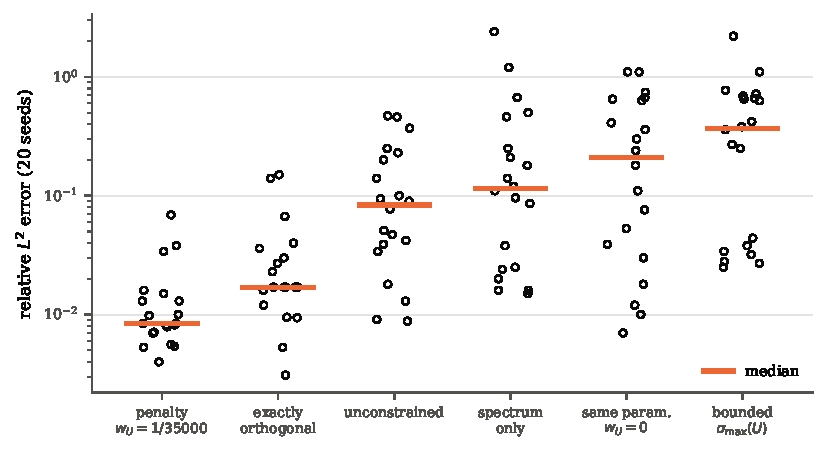
\includegraphics[width=0.75\textwidth]{fig_advection.pdf}
\caption{Per-seed relative error on the advection case, 20 seeds per regime,
log scale, ordered by median. The distributions are heavy-tailed and overlap
heavily, which is why medians are quoted alongside means. Bounding
$\sigma_{\max}(U)$ --- the weaker constraint predicted to substitute for the
penalty --- is the worst regime, below even removing the penalty outright.}
\label{fig:advection}
\end{figure}

\subsection{What the penalty does to the trained factors}

The source paper reports errors, not factor geometry. We measure, per
factorised layer of trained networks over 3 seeds, the orthogonality defect
$\DU = \|U^\top U - I\|_2$ and the largest relative gap between the trained
$|s|$ and the singular values of the effective weight $USV^\top$
(Table~\ref{tab:diagnostic}).

\begin{table}[htbp]
\centering
\caption{Factor geometry after training, 3 seeds, median over layers. If the
described mechanism held, $\DU$ would be near zero and the two spectra would
coincide. The bounded regime is discussed in Section~\ref{sec:bounded}; note
that it matches the penalised regime's $\DU$ while missing the spectrum by two
further orders of magnitude.}
\label{tab:diagnostic}
\begin{tabular}{lccc}
\toprule
Setting & Median error & Median $\DU$ & $|s|$ vs.\ true singular values \\
\midrule
$\wU = 1/35000$ & $7.9\times10^{-3}$ & $0.98$ & up to $13\times$ apart \\
$\wU = 0$       & $3.05\times10^{-1}$ & $63$ (max 177) & up to $31\times$ apart \\
Bounded $\sigma_{\max}(U)$ & $3.8\times10^{-1}$ & $1.00$ & up to $1290\times$ apart \\
\bottomrule
\end{tabular}
\end{table}

At the published weight $\DU \approx 1$, which for a defect measured in the
2-norm means an eigendirection of $U^\top U$ has collapsed: the trained factor
is rank-deficient, not near-orthogonal. The trained $s$ is not the effective
weight's spectrum. Both premises of the stated mechanism fail, while the
method's accuracy advantage holds.

Ordering the regimes by median error gives unconstrained-parameterised
$2.1\times10^{-1}$, spectrum-only $1.2\times10^{-1}$, unconstrained
$8.4\times10^{-2}$, exactly orthogonal $1.7\times10^{-2}$, weakly penalised
$8.4\times10^{-3}$. The penalty is doing something the method needs: removing
it lets the defect grow by two orders of magnitude and destroys the gain, while
enforcing the constraint it nominally approximates recovers only about half of
it. Exact orthogonality is a stronger constraint than the problem wants. The
natural reading is that the term bounds the scale of $U$ rather than
orthogonalising it, and Section~\ref{sec:bounded} tests that reading
directly --- it does not survive.

This reframes the first stated limitation: the open question is not how to
adapt $\wU$ but which constraint class the term belongs to. The ordering above
suggested that a bound weaker than orthogonality --- a cap on $U$'s largest
singular value, or a box on all of them --- should recover the gain without a
tuned penalty. We implemented the first of those, and it does not.

\subsection{Testing the prediction: bounding the largest singular value}
\label{sec:bounded}

The bounded regime rescales $U$ on every forward pass so that
$\sigma_{\max}(U) = 1$, leaving the remaining singular values free in $[0,1]$.
It is strictly weaker than orthogonality, which fixes all of them at 1, and it
admits the rank-deficient factor the penalty was measured to produce. It
carries no penalty term and no $\wU$. The scale it removes is not lost to the
layer, since $W = U\,\mathrm{diag}(s)\,V^\top$ and $s$ is trained.

Over 20 seeds it reaches $(4.68\pm5.1)\times10^{-1}$ mean and
$3.7\times10^{-1}$ median relative error: the worst of the six regimes, below
even the unpenalised parameterisation. The prediction is refuted.

Measuring the bounded networks' factors explains the failure and corrects our
earlier reading (last row of Table~\ref{tab:diagnostic}). The bounded regime
reaches $\DU = 1.00$, essentially the same defect as the penalised regime's
$0.98$ --- so on the statistic we used to characterise the penalty, the two are
indistinguishable. They are not indistinguishable in behaviour: the gap between
the trained $|s|$ and the effective weight's singular values is $13\times$ under
the penalty and $1290\times$ under the cap, and the bounded networks drive their
smallest trained singular value to $0$ exactly.

The reason is that $\DU = \max_i |\sigma_i(U)^2 - 1|$ saturates as soon as a
single direction of $U$ collapses, so it cannot distinguish one collapsed
direction from many. Capping $\sigma_{\max}(U)$ reproduces the value of $\DU$
while leaving the rest of the spectrum free to collapse, and the effective
weight then has nothing to do with the spectrum $s$ nominally controls. The
conclusion is narrower than the one we drew from the accuracy ordering alone:
what the penalty supplies is not a bound on the factor's scale --- a bound on
scale is exactly what the cap provides, and it fails --- and $\DU$ is too coarse
a summary to say what it is instead. Section~\ref{sec:mechanism}'s reading was
underdetermined by its own evidence.

The other half of the prediction --- a box holding every singular value of $U$
in $[1-\varepsilon, 1+\varepsilon]$ --- follows from that reading and is
untested. It is the constraint class that matches the measured behaviour, with
$\varepsilon$ a geometrically interpretable knob in place of a loss weight on
an unnormalised penalty, and it is the experiment we would run next.

The evidence here is one smooth one-dimensional problem, one architecture and
one optimiser. Whether the ordering survives on a shock is a separate
question, which is what Section~\ref{sec:swe} asks.

\section{Shallow-water dam breaks}
\label{sec:swe}

\subsection{Setup}

The benchmarks are two-dimensional dam breaks over a Gaussian-hump bed at the
conventions of the comparative study of Zahra
et al.~\cite{dambreak2026comparative}: domain $[0,100]^2$~m,
$g = 2$~m/s$^2$, reflective walls on all four sides, $t_{\text{end}} = 2$~s.
We use a step release, a circular column over a wet bed, the same column over
a dry bed, and a smooth Gaussian mound, all with Manning $n = 0$. A fifth
case, three submerged humps with Manning friction over 20~s, is included and
then set aside for the reason given below. Errors are
$L^1$ and $L^2$ of depth at the final output time on a shared $128^2$
evaluation grid, against a reference computed in-process with an HLLC
MUSCL--van Leer finite-volume scheme~\cite{toro2009riemann} at $512^2$ with
hydrostatic reconstruction for well-balancing~\cite{audusse2004wellbalanced}.
Baselines are an unmodified network, a Fourier-feature network --- the
standard remedy for high-frequency targets, absent from the source paper's
comparison --- and a finite-volume-informed network. Five seeds per cell.

Every strong-form entry is a 6-layer, 128-unit tanh network mapping
$(x,y,t)$ to primitive variables $(h,u,v)$, trained by Adam at $10^{-3}$ for
20000 iterations with gradient clipping at 1.0, on 20000 collocation points
resampled each step, with the initial condition imposed as a penalty at every
cell centre weighted 10 against the residual. Following the source paper, the
input and output layers stay dense and only the square hidden weights are
factorised. The Fourier-feature baseline uses 32 frequencies. The
finite-volume-informed entry predicts cell averages on the solver grid at 41
collocation times and is trained against the residual of the discrete SSP-RK2
update.

\subsection{Results}

Table~\ref{tab:matrix} gives all five benchmarks, five seeds each. On the
three shock-dominated cases no spectral regime separates from an unmodified
network by more than about 10\% in $L^1$ depth: on the step release every
entry but the finite-volume-informed one falls between $1.03$ and
$1.13\times10^3$, inside the unconstrained baseline's own seed spread. The
unconstrained network sits a factor of $4.1$ to $4.4$ above a classical scheme
at the same resolution.

\begin{table}[htbp]
\centering\small
\caption{$L^1$ depth error at the final output time on the $128^2$ evaluation
grid, mean $\pm$ s.d.\ over 5 seeds. Each column carries its own factor.
Section~\ref{sec:refcheck} gives the reference uncertainty for the wet,
step and Gaussian columns; it exceeds several of the differences here.}
\label{tab:matrix}
\begin{tabular}{lccccc}
\toprule
 & Circular, wet & Circular, dry & Step & Gaussian mound & Three humps \\
Entry & ($\times10^{3}$) & ($\times10^{3}$) & ($\times10^{3}$) & ($\times10^{2}$) & ($\times10^{2}$) \\
\midrule
Classical, $128^2$ & $0.391$ & $0.380$ & $0.248$ & $0.064$ & $0.797$ \\
\midrule
Unconstrained      & $1.602\pm0.012$ & $1.681\pm0.076$ & $1.028\pm0.11$  & $3.83\pm0.22$ & $8.87\pm0.68$ \\
Fourier features   & $1.681\pm0.11$  & $1.838\pm0.12$  & $1.124\pm0.068$ & $4.03\pm0.48$ & $7.96\pm1.5$ \\
Penalised spectral & $1.662\pm0.12$  & $1.602\pm0.054$ & $1.106\pm0.047$ & $4.69\pm0.55$ & $7.49\pm1.1$ \\
Exactly orthogonal & $1.725\pm0.13$  & $1.507\pm0.14$  & $1.054\pm0.071$ & $9.69\pm1.8$  & $9.19\pm2.3$ \\
Spectrum only      & $2.347\pm0.11$  & $2.314\pm0.19$  & $1.126\pm0.015$ & $9.16\pm0.34$ & $6.08\pm1.1$ \\
FV-informed        & $14.81\pm2.4$   & $9.32\pm0.54$   & $13.65\pm2.7$   & $44.0\pm5.6$  & $8.66\pm0.22$ \\
\bottomrule
\end{tabular}
\end{table}

The two benchmarks that do separate separate against the method. On the
Gaussian mound --- the only smooth initial condition in the set, and the case
closest to the regime the source paper validates in --- exact orthogonality
reaches $(9.69\pm1.8)\times10^2$ against the unconstrained network's
$(3.83\pm0.22)\times10^2$, and spectrum-only training $(9.16\pm0.34)\times10^2$.
That is a factor of $2.5$ in the wrong direction, it is far outside the seed
spread, and Section~\ref{sec:refcheck} puts the reference uncertainty on this
benchmark at $3.8\times10^2$, so the gap is resolvable where smaller ones are
not. The penalised regime is intermediate at $(4.69\pm0.55)\times10^2$.
Constraining the factor hurts most where the target is smooth.

On the three-hump case with Manning friction the ordering inverts:
spectrum-only training is the best neural entry at $(6.08\pm1.1)\times10^2$
and exact orthogonality the worst at $(9.19\pm2.3)\times10^2$. We do not read
this as support for the spectral family, because every entry on that benchmark
loses between 63\% and 90\% of its initial mass over the 20~s run --- against
$10^{-3}$ or below on the two-second cases --- so all six models are far
outside any regime where a depth error is meaningful. The case is reported for
completeness and should not be used to rank methods.

The finite-volume-informed network collapses on the four short cases, matching
the behaviour reported for it in~\cite{dambreak2026comparative}.


\begin{figure}[htbp]
\centering
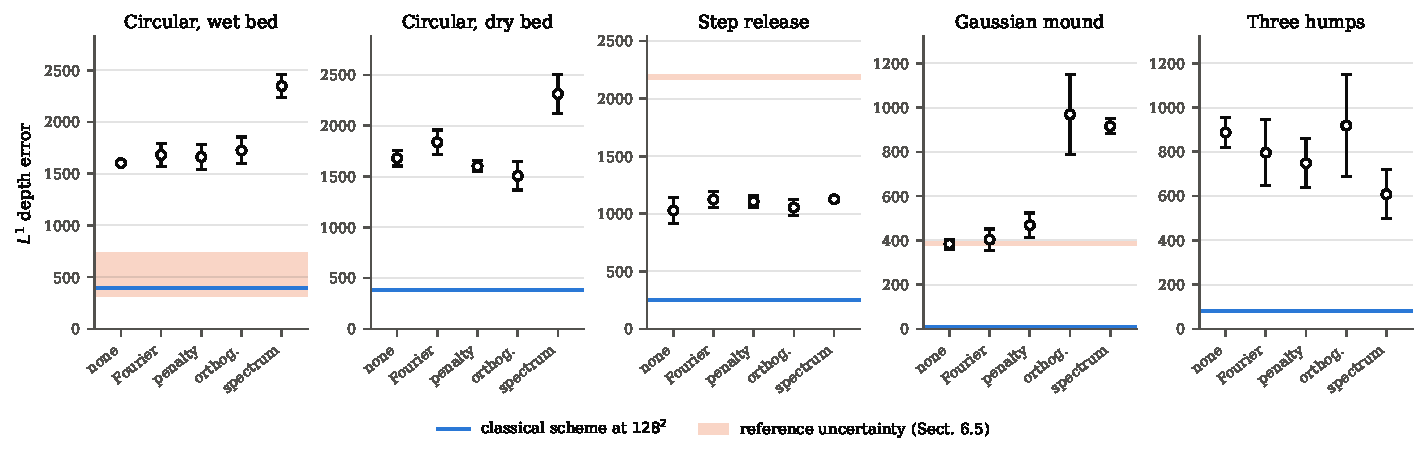
\includegraphics[width=\textwidth]{fig_matrix.pdf}
\caption{$L^1$ depth error by benchmark, mean $\pm$ s.d.\ over 5 seeds; the
finite-volume-informed entry is off-scale and omitted. The blue line is a
classical scheme at the evaluation resolution. The orange band, where present,
spans the disagreement between our reference and two independently implemented
schemes on the same initial condition (Section~\ref{sec:refcheck}); on the step
release it sits above every neural result, and on the Gaussian mound it is the
width of the vanilla network's own error. Only the Gaussian mound separates the
regimes, and it separates them against the constrained ones.}
\label{fig:matrix}
\end{figure}

\subsection{Does the penalty weight matter here?}
\label{sec:sweep}

The first of the source paper's stated limitations is that $\wU$ must be tuned
per equation, and no published value exists for shallow-water flow. We
bracketed it over three decades on the two circular benchmarks with the
corrected Eq.~\eqref{eq:penalty} penalty, five seeds per cell
(Table~\ref{tab:sweep}).

\begin{table}[htbp]
\centering
\caption{$L^1$ depth error against $\wU$ over three decades, five seeds,
using the 2-norm penalty of Eq.~\eqref{eq:penalty}. The spread across the
whole range is smaller than the spread across seeds within any one cell.}
\label{tab:sweep}
\begin{tabular}{lcc}
\toprule
$\wU$ & Circular, wet bed & Circular, dry bed \\
\midrule
$10^{-3}$            & $(1.578\pm0.025)\times10^{3}$ & $(1.765\pm0.032)\times10^{3}$ \\
$1/35000 = 2.9\times10^{-5}$ & $(1.601\pm0.12)\times10^{3}$ & $(1.709\pm0.056)\times10^{3}$ \\
$10^{-6}$            & $(1.549\pm0.069)\times10^{3}$ & $(1.643\pm0.050)\times10^{3}$ \\
\bottomrule
\end{tabular}
\end{table}

Three orders of magnitude in $\wU$ move the error by 3\% on the wet bed and
7\% on the dry bed, both inside the seed-to-seed spread. On these problems
the tuning burden the source paper identifies does not exist, because the
knob does not do anything. That is a negative answer to their first
limitation in this regime rather than a solution to it: there is nothing to
adapt. It also says the penalty is not the active ingredient here, which is
consistent with the whole spectral family sitting within 10\% of an
unmodified network on the same benchmarks.

This sweep supersedes one reading we drew from the earlier, Frobenius-penalty
run and now retract. There, the penalised network placed the radial front on
the dry bed at $3.5\pm4.1$~m from the reference against the unconstrained
network's $21.2\pm8.6$~m, which we took as a local advantage invisible to the
integrated error. Under the corrected penalty the same quantity is
$14.8\pm6.6$~m at $\wU = 1/35000$ and between $14.8$ and $17.0$~m across the
three decades, overlapping the unconstrained baseline within one standard
deviation. The apparent front-position advantage belonged to the stronger
Frobenius penalty, not to the published method, and it does not survive.
Integrated depth error was almost unaffected by the same change
($1.662\times10^3$ against $1.601\times10^3$ on the wet bed), so the norm
choice matters for where the shock is placed and not for the depth field as a
whole.

\subsection{What the regimes cost}
\label{sec:cost}

The second stated limitation is the penalty's training overhead, which the
source paper puts at 1.28 to 1.83 times vanilla across its width and
collocation sweeps. Table~\ref{tab:cost} gives wall-clock training time over
all 25 runs per entry on one Quadro RTX 8000.

\begin{table}[htbp]
\centering
\caption{Mean training time per run, 25 runs per entry (5 benchmarks $\times$
5 seeds), identical iteration budgets. The penalty is nearly free here; the
penalty-free alternative is the expensive one.}
\label{tab:cost}
\begin{tabular}{lcc}
\toprule
Entry & Mean training time (s) & Relative to unconstrained \\
\midrule
Unconstrained      & 861 & $1.00\times$ \\
Spectrum only      & 862 & $1.00\times$ \\
Penalised spectral & 884 & $1.03\times$ \\
Fourier features   & 946 & $1.10\times$ \\
Exactly orthogonal & 1226 & $1.42\times$ \\
FV-informed        & 2048 & $2.38\times$ \\
\bottomrule
\end{tabular}
\end{table}

The overhead the source paper reports does not reproduce in this setting: the
penalty costs 3\%, not 28--83\%. One 2-norm of a $128\times128$ matrix per
factorised layer per step is negligible against 20000 collocation points, and
we suspect the published figures reflect a smaller problem where the penalty
is a larger share of the step, or a different implementation of the norm.

The direction of the comparison matters more than the absolute numbers.
Removing the penalty by constraining the factor exactly costs 42\%, because
the matrix-exponential retraction runs on every forward pass. So on cost
grounds the penalty-free route is worse than the penalty, not better, and the
motivation for eliminating $\wU$ has to rest on the tuning burden alone ---
which Section~\ref{sec:sweep} shows does not exist on these problems either.
Spectrum-only training is free relative to the baseline, as expected from
training $n$ parameters per layer instead of $n^2$, but it buys nothing in
accuracy.


\subsection{How far the reference can be trusted}
\label{sec:refcheck}

Every number in Table~\ref{tab:matrix} is measured against one solver's output.
To find out what that is worth, we compare the reference against an
independent implementation: the HLL, Lax--Wendroff and MUSCL--Rusanov runs
produced for~\cite{dambreak2026comparative} on a $501^2$ node grid for the
same initial conditions, interpolated onto the evaluation grid. Those runs
store depth only, so the comparison is on depth.

\begin{table}[htbp]
\centering
\caption{$L^1$ depth disagreement between our $512^2$ HLLC reference and three
independently implemented schemes on the same initial condition, against our
own discretisation error and the unconstrained network's error. Read down a
column: where the middle entries exceed the last, the benchmark cannot resolve
differences of the size Table~\ref{tab:matrix} reports.}
\label{tab:crosscheck}
\begin{tabular}{lccc}
\toprule
 & Circular, wet bed & Gaussian mound & Step release \\
\midrule
Our classical at $128^2$      & $3.914\times10^{2}$ & $6.357\times10^{0}$ & $2.476\times10^{2}$ \\
\midrule
vs.\ their HLL                & $3.111\times10^{2}$ & $3.763\times10^{2}$ & $2.169\times10^{3}$ \\
vs.\ their MUSCL--Rusanov     & $7.395\times10^{2}$ & $3.949\times10^{2}$ & $2.208\times10^{3}$ \\
vs.\ their Lax--Wendroff      & $7.551\times10^{3}$ & $3.435\times10^{3}$ & $9.349\times10^{3}$ \\
\midrule
Unconstrained network         & $1.602\times10^{3}$ & ${\sim}3.9\times10^{2}$ & $1.028\times10^{3}$ \\
\bottomrule
\end{tabular}
\end{table}

Three regimes appear. On the wet-bed column the reference is vindicated: it
agrees with an independent HLL implementation to $3.11\times10^2$, tighter
than its own $128^2$ discretisation error of $3.91\times10^2$, and both are
far below the $1.60\times10^3$ network error. Differences between network
variants on that benchmark are real. On the Gaussian mound the two solver
families disagree by $3.76\times10^2$ and the network error is
$3.9\times10^2$ --- the same number --- while our own discretisation error is
sixty times smaller at $6.36$. On the step release the solver families differ
by $2.2\times10^3$, twice the network error. No ranking of network variants on
those two benchmarks survives a change of reference solver.

Lax--Wendroff is the outlier throughout, which is expected of Lax--Wendroff
with artificial viscosity at a shock and is a statement about that scheme
rather than about ours. Nothing here says our reference is wrong; it is the
most refined and least diffusive of the four, and on the wet-bed column it is
confirmed. What it says is that a comparison table of this kind has a
resolution floor that varies by benchmark, and that the floor has to be
quoted next to any margin claimed from it. We have not seen this check
performed in the PINN-for-conservation-laws literature, where a single
fine-grid run is the usual reference.

\section{Limitations}

Five seeds per cell resolve a factor of two, not the 10\% differences that
make up most of Table~\ref{tab:matrix}; only the Gaussian-mound column
separates by more than the spread. Section~\ref{sec:refcheck} bounds what the
comparison can resolve at all and should be read before
Table~\ref{tab:matrix}, not after it. The three-hump case is reported but not
interpretable: every model there loses most of its mass.

The factor-geometry measurement of Table~\ref{tab:diagnostic} uses 3 seeds on
one one-dimensional problem, one architecture and one optimiser, and it is the
basis for the paper's central claim about what the penalty does. It should be
repeated on the shallow-water networks, where the per-run factor diagnostics
are now recorded but not yet analysed.

The singular-value box of Section~\ref{sec:bounded}, which is what the refuted
prediction points to, is not implemented. Until it is, the claim that the
penalty acts by pulling the whole spectrum toward 1 rests on one measurement
of $D$ and one failed alternative, both on the advection case.

Two of the five contributions in the project proposal have no section here.
The pointwise condition-number field, which is the diagnostic that would
explain \emph{where} on the shock the spectral variants fail rather than only
that they do, is not built. Neither is the Navier--Stokes leg --- the
Taylor--Green case the source paper reports and the lid-driven cavity --- which
is what would connect these results back to the setting~\cite{wang2026cnpinn}
validates in. Cost and memory were recorded per run but are not tabulated, so
the second stated limitation of the source paper is not yet answered
quantitatively.

\section{Conclusion}

The orthogonality penalty of~\cite{wang2026cnpinn} is load-bearing on their
own advection problem and is not doing what the paper says it does. At the
published weight the trained factor is rank-deficient rather than orthogonal,
and the trained singular values are not the effective weight's spectrum, yet
removing the penalty destroys the accuracy gain and enforcing exact
orthogonality recovers only about half of it. Replacing the penalty with a
bound on the factor's largest singular value --- the weaker constraint that
reading suggests --- is the worst of the six regimes we tried. That rules the
scale-bound reading out rather than replacing it: the bounded networks match
the penalised ones on the orthogonality defect $\DU$ while missing the
effective spectrum by two further orders of magnitude, so $\DU$ is too coarse
a statistic to characterise what the penalty does, and what it does instead
remains open.

Moving to shock-dominated shallow-water flow, outside the reach of the source
paper's Theorem 2.1, the picture is flatter and in one place reversed. On the
three shock cases no spectral regime separates from an unmodified network by
more than about 10\% in integrated depth error, and the penalty weight can be
moved three decades without measurable effect, so the tuning problem the
source paper poses does not arise. On the one smooth case in the set, exact
orthogonality and spectrum-only training are a factor of $2.5$ \emph{worse}
than an unmodified network, by a margin that exceeds the reference
uncertainty. Whatever the reparameterisation contributes on smooth
one-dimensional targets does not transfer, and constraining the factor
hurts most where the target is smoothest.

Establishing any of this required checking the reference against an
independent solver family, which on two of three benchmarks disagrees with it
by more than the differences under test. We would encourage that check as
routine practice: a single fine-grid run is the usual reference in this
literature, and its uncertainty is rarely quoted.

\bibliographystyle{plain}
\bibliography{references}

\end{document}
